Pour comprendre le manuscrit dans son intégralité, il sera nécessaire de comprendre quelques outils.
Ces outils n'entrant pas dans le récis de la thèse, j'ai choisi de les décrire dans cette section de prérequis.
Premiérement, nous allons décrire le format de représentation moléculaire que nous allons utiliser tout au long du manuscrit, puis nous expliquerons ensuite l'outil mathématique que sont les graphes.

\section{Chimie et SMILES}

\subsection{Représentation 2D de molécules}

\begin{figure}[h!]
  \begin{center}
    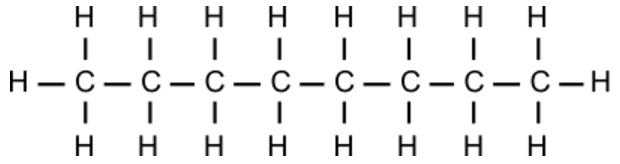
\includegraphics[width=300px]{Figures/Prerequis/developpee.png}
    \caption{\label{dev}Formule développée de la molécule d'octane.}
  \end{center}
\end{figure}

L'ensemble du manuscrit va parler de molécules issues de constructions biologiques.
Une molécule peut classiquement être représentée en 2D sous la forme d'un dessin d'atomes représentés par des lettres, liées par des traits représentant les liaisons covalentes entre atomes (voir figure \ref{dev}).
Cette représentation est appelée formule développée de la molécule.

\begin{figure}[h!]
  \begin{center}
    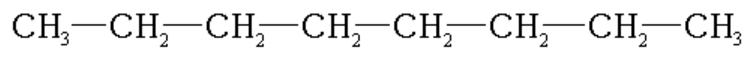
\includegraphics[width=300px]{Figures/Prerequis/semi.png}
    \caption{\label{semi}Formule semi-développée de la molécule d'octane.}
  \end{center}
\end{figure}

Les atomes d'hydrogène étant présents partout, la représentation de molécules conséquentes devient rapidement lourde.
C'est dans le but de simplifier les représentations qu'à été inventée la formule semi-développée (voir figure \ref{semi}).
Les atomes d'hydrogène n'effectuant qu'une seule liaison peuvent être contracté avec l'atome qu'ils accompagne sans pour autant avoir un doute sur les liaisons non dessinées.


\subsection{Représentation 1D d'une molécule : les SMILES}

Les librairies de chemoinformatique utilisent un format plus compacte pour les représentations moléculaires.
Toute la structure est compactée en un texte en une seule dimension.
Ce format est appelé SMILES (pour \textit{Simplified Molecular Input Line Entry Specification}) et a été publié en 1988~\cite{weininger_smiles_1988}.
L'octane représenté plus haut sera par exemple écrit sous la forme :

\[\text{[C]([H])([H])([H])[C]([H])([H])[C]([H])([H])[C]([H])([H])[C]([H])([H])[C]([H])([H])}\]
\[\text{[C]([H])([H])[C]([H])([H])[H]}\]

Chaque atome est représentée par une lettre entourée de crochets.
Deux atomes directement à la suite l'un de l'autre sont considérés comme liés.
Une sous partie de l'expession entre parenthèse représente un embranchement à partir de l'atome précédent.
Sur cet exemple, la chaîne principale est donc constituée de [C][C][C][C][C][C][C][C][H].
Chacun des [C] est accompagné de plusieurs branchements ne contenant qu'un seul hydrogène.
Par exemple le début de la chaîne est constituée d'un [C]([H])([H])([H]), ce qui veut dire que que le carbone, en plus d'être lié au carbone suivant, possède trois branches contenant chacune un hydrogène.
Il est à noter qu'il existe de nombreux SMILES pour cette molécule.
J'ai arbitrairement choisi de commencer par le carbonne tout à gauche, mais pu démarrer du milieu.

La notation présentée est lourde mais est allégée par deux règles supplémentaires.
Premiérement, les atomes d'hydrogène sont facultatifs.
Même si ils ne sont pas présents dans l'écriture, ils seront automatiquement ajoutés jusqu'à saturation des atomes hôtes.
Pour représenté un atome n'étant pas totalement saturé en hydrogène, il faudra lui ajouter les symboles ioniques + ou -.
Ainsi, un [C-] représentera un carbone dont un des électrons de la couche de valence est encore libre pour une liaison.
Deuxiémement, il est autoriser de ne pas mettre les crochets pour les atomes les plus fréquemment utilisés en chimie organisque (par exemple C, N ou O).
Avec ces deux assouplissements notre molécule d'octane s'écrirait donc de la manière suivante : CCCCCCCC.

Les SMILES doivent inclure plusieurs autres règles pour pouvoir représenter l'intégralité des molécules possibles.
Ainsi, un = ou un \# sont ajoutés entre deux atomes pour représenter des liaisons doubles et triples.
Par exemple, le SMILES C(=O)OH représente un groupement carboxyle.
Le =O est une branche reliée au C par une double liaison.

\begin{figure}[h!]
  \begin{center}
    
\includegraphics[width=110px]{Figures/Prerequis/glucose.png}
    \caption{\label{glucose}Molécule de glucose.}
  \end{center}
\end{figure}

Les molécules peuvent également être cycliques.
Il n'est pas possible de représenter un cycle dans un texte sans ajouter de notation.
Ainsi, on ajoute un nombre à la suite de deux atomes distants dans la chaîne qui doivent être reliés.
La molécule de glucose représentée sur la figure \ref{glucose} s'écrira donc OCC1C(O)C(O)C(O)C(O)O1.

Je n'ai décrit ici que les règles qui nous seront utiles.
L'intégralité des spécifications est disponible en ligne sur de nombreux sites.



\section{Graphes}





























